% Copyright (C) 2012-2020 Dmitry V. Levin <ldv@altlinux.org>
% Copyright (C) 2023 Eugene Syromiatnikov <evgsyr@gmail.com>
% Permission is granted to copy, distribute and/or modify this document
% under the terms of the GNU Free Documentation License, Version 1.2
% or any later version published by the Free Software Foundation;
% with no Invariant Sections, no Front-Cover Texts, and no Back-Cover Texts.

\documentclass[unicode,aspectratio=169]{beamer}

\mode<presentation>
{
	\usetheme{Warsaw}
	\setbeamertemplate{headline}{}
	\setbeamertemplate{footline}{\hfill \insertframenumber/\inserttotalframenumber}
	\setbeamertemplate{navigation symbols}{}
}

\usepackage[utf8]{inputenc}
\usepackage[T2A]{fontenc}
\usepackage[english]{babel}
\usepackage{alltt}
\usepackage{verbatim}
\usepackage{hyperref}
\usepackage{listings}
\lstset{
basicstyle=\scriptsize\ttfamily,
columns=flexible,
breaklines=true
}

\pgfdeclareimage[height=1.2cm]{right-corner-logo}{strace-straus.pdf}
\pgfdeclareimage[height=8cm]{strace-logo}{strace-straus.pdf}

\title{\Huge netlink decoding in strace}
\author{\Huge Eugene~Syromiatnikov}
\date{\Large DevConf.cz, 2023}

\logo{\pgfuseimage{right-corner-logo}}

\begin{document}

%%%%%%%
{
\setbeamertemplate{footline}{}
\begin{frame}[noframenumbering]
\titlepage
\end{frame}
}

%%%%%%%
\begin{frame}{What is \texttt{strace}?}
\begin{quote}
\texttt{strace} is a diagnostic, debugging and instructional userspace
utility for Linux.
It is used to monitor and tamper with interactions between processes
and the Linux kernel, which include system calls, signal deliveries,
and changes of process state.

\begin{flushright}
— \url{https://strace.io/}
\end{flushright}
\end{quote}
\end{frame}

%%%%%%%
\begin{frame}{Interaction between processes and the Linux kernel}
Over the years, the interaction between userspace processes and the kernel becomes more and more diverse:
\begin{itemize}
  \item various "dispatcher syscalls", like \texttt{fcntl(2)}, \texttt{prctl(2)}, \texttt{[gs]etsockopt(2)} or \texttt{ioctl(2)}, that have no strongly defined symantics;
  \item \texttt{msg\_control} field of \texttt{struct msghdr};
  \item virtual file systems, most notoriously \texttt{procfs}, but also \texttt{sysfs}, \texttt{security}/\texttt{selinux}, \texttt{bpf}, ...;
  \item special file descriptors: \texttt{fanotify\_init(2)}, \texttt{signalfd(2)};
  \item \texttt{io\_uring(2)};
  \item virtual address families: \texttt{AF\_NETLINK}, \texttt{AF\_ALG}, \texttt{AF\_XDP};
  \item ...
\end{itemize}
\end{frame}

%%%%%%%
\begin{frame}{\texttt{ioctl(2)}}
\begin{itemize}
  \item \texttt{ioctl(int fd, unsigned long request, ...)}
  \item Historically, a way to manipulate devices associated with special files
  \item Acts as "catch-all" for many, many kinds of kernel interactions
  \begin{itemize}
    \item \emph{Just create some device file, add some ioctl(2) handler for it, and off you go}
  \end{itemize}
  \item Used to control file descriptor (so, \texttt{fcntl(2)} then?),
        inode properties and attributes (not to be confused
        with \texttt{\{list,set,del\}xattr}, especially
	\texttt{FS\_IOC\_FS[GS]ETXATTR}), FS properties
  \item terminals, block devices, MTD, evdev, V4L2, LIRC, GPIO, NBD, SCSI,
        watchdog, RTC, TEE, device mapper;  seccomp, UFFD, perf, inotify, KVM,
	...
\end{itemize}
\end{frame}

%%%%%%%
\begin{frame}{Issues with \texttt{ioctl(2)} as an interface}
\begin{itemize}
  \item No specification with regards to anything: how \texttt{request}
        is encoded and used, how the argument is interpreted
  \begin{itemize}
    \item There is \texttt{\_IOC(dir, type, ns, size)} macro for constructing
          \texttt{request}  numbers, but it is not universally used,
	  and, to add insult to the injury, it is arch-dependent
  \end{itemize}
  \item Which is especially fun in case of file descriptors associated
        with complex stacks (like storage or networking), where each layer
        can and has its own set of ioctl requests
  \item Basically, everything is up to the implementation, which leads
        to constantly recurring issues, such as:
  \begin{itemize}
    \item No proper support or breakage of compat (32-on-64-bit) processes
          or peculiar architectures (hi, m68k!)
          due to variability of type sizes or alignment rules between them
    \item Issues with extending of the structures that are passed to/from
          the kernel (or starting using parts of them), which leads to all
	  these wonderful\footnotemark[1] \texttt{KDFONTOP}
	  and \texttt{GPIO\_V2\_*} requests
  \end{itemize}
\end{itemize}
\footnotetext[1]{Of course, this is not exclusive to \texttt{ioctl(2)} interface per se, as existence of various \texttt{faccessat2(2)}, \texttt{statx(2)}, or \texttt{FUTEX\_LOCK\_PI2} might indicate}
\end{frame}

%%%%%%%
\begin{frame}{Netlink: "a better \texttt{ioctl(2)}" (?)}
\begin{itemize}
  \item Wire protocol for communicating between the user space and the kernel
  \item \texttt{socket(AF\_NETLINK, SOCK\_RAW, \textit{netlink\_proto});}
  \begin{itemize}
    \item No longer requiring obtaining of a file descriptor for the operation
          (which was somewhat artificial in some cases)
  \end{itemize}
  \item Header (or multiple headers, in some cases) + hierarchy of attributes,
        every part is of known size and type, since they are passed
	in the associated header
  \item Reservations for various types of communications (in reality, other
        than single request-response communications, only asynchronous
	notifications are used so far)
  \item Kernel infrastructure in place for parsing netlink messages
        in accordance with policies that have provisions for various data types
  \item Several existing interfaces (iproute/netfilter, ethtool, NBD) have
        switched from \texttt{ioctl(2)}-based interfaces to netlink-based ones
  \item Many new kernel interfaces are initially implemented using netlink
        (taskstats, DRBD, thermal)
\end{itemize}
\end{frame}

%%%%%%%
\begin{frame}{Support for netlink in strace: some history}
\begin{itemize}
  \item Initial implementation of general netlink decoding was done as part
        of GSoC 2016 project by Fabien Siron and is available since strace 4.13;
  \item It got significantly extended as part of GSoC 2017 project
        by Chen Jingpiao, and was made available as part of strace 4.18
	and strace 4.19 releases;
  \item Since then, netlink decoding in strace has been receiving various
        updates, in part in the form of adding support for new attribute types
	added in the kernel, in part as more thorough implementation
	of decoding of some message and attribute types.
\end{itemize}
\end{frame}

%%%%%%%
\begin{frame}{Support for netlink in strace: implementation}
\begin{itemize}
  \item Entry point, \texttt{decode\_netlink()}, is hooked into \texttt{send(2)}
        decoder and \texttt{print\_struct\_msghdr} printer, replacing simple
        string printing when the protocol name associated with the socket
        is "NETLINK" or when the address family in the \texttt{msg\_name}
        field is \texttt{AF\_NETLINK}, respectively
  \item The whole decoding is progressive and is mostly a cascade
        of decoder-table-driven calls: specific decoder parses the header
        and then dispatches payload decoding based on message/attribute type
        using the decoder table, for example:
  \begin{itemize}
    \item \texttt{netlink.c:decode\_netlink()} calls
          \texttt{decode\_nlmsghdr\_with\_payload()};
    \item \texttt{netlink.c:decode\_nlmsghdr\_with\_payload()} calls
          \texttt{decode\_payload()};
    \item \texttt{netlink.c:decode\_payload()} calls
          \texttt{netlink\_decoders[family]()};
    \item \texttt{netlink\_sock\_diag.c:decode\_netlink\_sock\_diag()} (pointer
          to which is at \texttt{netlink\_decoders[NETLINK\_SOCK\_DIAG]}) calls
          \texttt{diag\_decoders[family]};
    \item \texttt{netlink\_inet\_diag.c:decode\_inet\_diag\_msg()} (pointer
          to which is at \texttt{diag\_decoders[AF\_INET]}) calls
          \texttt{decode\_nlattr()}, passing \texttt{inet\_diag\_attrs} xlat
          and \texttt{inet\_diag\_msg\_nla\_decoders} decoder table to it;
    \item \texttt{nlattr.c:decode\_nlattr()} is a generic nested attribute
          decoder that handles a sequence of netlink attributes by calling
          a decoder from the decoder table according to the attribute type.
  \end{itemize}
\end{itemize}
\end{frame}

%%%%%%%
\begin{frame}[fragile]{Support for netlink in strace: testing \hfill (1/2)}
\begin{itemize}
  \item Testing is mostly done with respect to the expectedness of the decoder
        output on the various synthetic payloads, no attempts to parse
        the actual data from the kernel are made;
  \item A common test harness is used, where the test binary produces
        the expected output, which is then compared with the actual output
        \texttt{strace} (with the appropriate options) has produced during
        the run of the test binary;
  \item To aid the implementation of the tests (especially the synthesis
        of appropriately laid out test vectors), a number of macros
        and helper functions is present in \texttt{test\_netlink.h}
        and \texttt{test\_nlattr.h}.
\end{itemize}
\end{frame}

%%%%%%%
\begin{frame}[fragile]{Support for netlink in strace: testing \hfill (2/2)}
\begin{block}{Excerpt from \texttt{tests/nlattr\_tc\_stats.c}}
\begin{lstlisting}
        static const uint64_t pkt64 = 0xdeadc0defacefeedULL;
        TEST_NESTED_NLATTR_OBJECT(fd, nlh0, hdrlen, init_tcmsg, print_tcmsg,
          `      TCA_STATS_PKT64, pattern, pkt64, printf("16045693111314087661"));
\end{lstlisting}
\end{block}
\begin{block}{Excerpt from \texttt{tests/nlattr\_tc\_stats.dir/exp}}
\begin{lstlisting}
sendto(3, [{nlmsg_len=51, nlmsg_type=RTM_GETQDISC, nlmsg_flags=NLM_F_DUMP, nlmsg_seq=0, nlmsg_pid=0}, {tcm_family=AF_UNIX, tcm_ifindex=if_nametoindex("lo"), tcm_handle=0, tcm_parent=0, tcm_info=0}, [{nla_len=15, nla_type=TCA_STATS2}, [{nla_len=11, nla_type=TCA_STATS_PKT64}, "\x61\x62\x63\x64\x65\x66\x67"]]], 51, MSG_DONTWAIT, NULL, 0) = 51
sendto(3, [{nlmsg_len=52, nlmsg_type=RTM_GETQDISC, nlmsg_flags=NLM_F_DUMP, nlmsg_seq=0, nlmsg_pid=0}, {tcm_family=AF_UNIX, tcm_ifindex=if_nametoindex("lo"), tcm_handle=0, tcm_parent=0, tcm_info=0}, [{nla_len=16, nla_type=TCA_STATS2}, [{nla_len=12, nla_type=TCA_STATS_PKT64}, 0x7fcde6ce5ff9]]], 52, MSG_DONTWAIT, NULL, 0) = -1 EFAULT (Bad address)
sendto(3, [{nlmsg_len=52, nlmsg_type=RTM_GETQDISC, nlmsg_flags=NLM_F_DUMP, nlmsg_seq=0, nlmsg_pid=0}, {tcm_family=AF_UNIX, tcm_ifindex=if_nametoindex("lo"), tcm_handle=0, tcm_parent=0, tcm_info=0}, [{nla_len=16, nla_type=TCA_STATS2}, [{nla_len=12, nla_type=TCA_STATS_PKT64}, 16045693111314087661]]], 52, MSG_DONTWAIT, NULL, 0) = 52
\end{lstlisting}
\end{block}
\end{frame}

%%%%%%%
\begin{frame}[fragile]{Support for netlink in strace: example}
\begin{columns}
\column{10cm}
\begin{block}{\scriptsize\texttt{strace --syscall-limit=2 -erecvmsg -s2 -q ss -t> /dev/null}}
\begin{scriptsize}
\begin{lstlisting}
recvmsg(3, {msg_name={sa_family=AF_NETLINK, nl_pid=0, nl_groups=00000000}, msg_namelen=12, msg_iov=[{iov_base=NULL, iov_len=0}], msg_iovlen=1, msg_controllen=0, msg_flags=MSG_TRUNC}, MSG_PEEK|MSG_TRUNC) = 3224
recvmsg(3, {msg_name={sa_family=AF_NETLINK, nl_pid=0, nl_groups=00000000}, msg_namelen=12, msg_iov=[{iov_base=[[{nlmsg_len=124, nlmsg_type=SOCK_DIAG_BY_FAMILY, nlmsg_flags=NLM_F_MULTI, nlmsg_seq=123456, nlmsg_pid=19344}, {idiag_family=AF_INET, idiag_state=TCP_ESTABLISHED, idiag_timer=0, idiag_retrans=0, id={idiag_sport=htons(57454), idiag_dport=htons(5900), idiag_src=inet_addr("192.168.101.232"), idiag_dst=inet_addr("192.168.101.109"), idiag_if=0, idiag_cookie=[28676, 0]}, idiag_expires=0, idiag_rqueue=0, idiag_wqueue=0, idiag_uid=1000, idiag_inode=47703907}, [[{nla_len=5, nla_type=INET_DIAG_SHUTDOWN}, 0], ...]], ...], iov_len=32768}], msg_iovlen=1, msg_controllen=0, msg_flags=0}, 0) = 3224
\end{lstlisting}
\end{scriptsize}
\end{block}
\column{4cm}
{\centerline{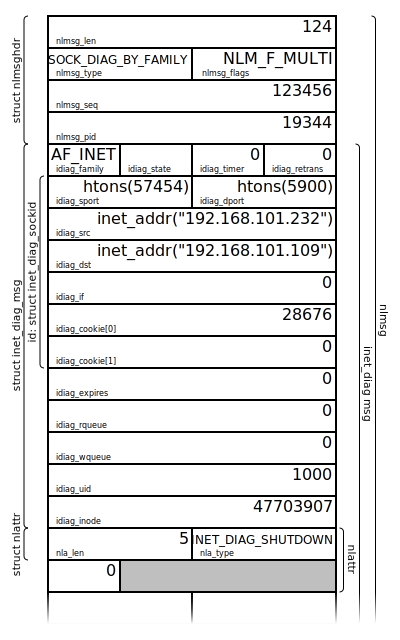
\includegraphics[height=6.4cm]{nlmsg_example.pdf}}}
\end{columns}
\end{frame}

%%%%%%%
\begin{frame}[fragile]{Support for netlink in strace: caveats \hfill (1/4)}
\begin{block}{Don't provide the necessary information for decoding}
\begin{itemize}
  \item \texttt{AF\_SMC}'s\footnotemark[1] \texttt{sock\_diag} implementation
        decided at some point\footnotemark[2] to put the underlying
	protocol (\texttt{AF\_INET}/\texttt{AF\_INET6}) instead of the actual
	address family name the message should be associated with.
  \item Made strace impossible to discern between \texttt{inet\_diag}
        and \texttt{smc\_diag} messages
  \item Fixed in Linux commit v5.1-rc1\~{}178\^{}2\~{}328\^{}2
  % Funnily, it haven't affected its main user, ss, because it doesn't request
  % sockets for all families at once, but rather performs a request for each
  % address family separately, probably in anticipation of such kind
  % of behaviour from the kernel code.
\end{itemize}
\end{block}
\footnotetext[1]{SMC stands for "shared memory communications (over RDMA)",
                 not to be confused  with RDS ("reliable datagram sockets")
		 over RDMA, XDP, or VSOCK (in case of SMC-D, which is used
		 for communications between a hypervisor and a guest)}
\footnotetext[2]{Around adding IPv6 support, see Linux commit v4.18-rc1\~{}114\^{}2\~{}323\^{}2\~{}2}
\end{frame}

%%%%%%%
\begin{frame}[fragile]{Support for netlink in strace: caveats \hfill (2/4)}
\begin{block}{Semantics of attributes depends on the value in other attributes}
\begin{itemize}
  \item There are multiple places in \texttt{NETLINK\_ROUTE}, for example,
        where there is a \texttt{*\_KIND} or \texttt{*\_AF\_SPEC} attribute that
        specifies the protocol/address family other attributes (or attributes
	within other attributes);
  \item Handled on case-by-case basis by tracking the last value
        of the determining attribute in a structure that is passed between
	the decoders of specific attributes.
\end{itemize}
\end{block}
\end{frame}

%%%%%%%
\begin{frame}[fragile]{Support for netlink in strace: caveats \hfill (3/4)}
\begin{block}{Using structures inside netlink attributes}
\begin{itemize}
  \item All the issues previously mentioned with respect to \texttt{ioctl(2)}
        requests' implementations, but now inside netlink attributes!
  \item One of the later fixes: v5.3-rc7\~{}29\^{}2\~{}35\^{}2\~{}1 "netfilter: xt\_nfacct:
        Fix alignment mismatch in xt\_nfacct\_match\_info"
  \item From the point of the decoder, the only discriminator present
        is the attribute's size, but, most of the time, it is enough.
\end{itemize}
\end{block}
\begin{block}{Using attribute types as array indices}
\begin{itemize}
  \item That is outright ignoring of the netlink spec that states that
        \texttt{nla\_type} determines attribute semantics.
  \item Required special-casing in \texttt{decode\_nlattr()} implementation.
\end{itemize}
\end{block}
\end{frame}

%%%%%%%
\begin{frame}[fragile]{Support for netlink in strace: caveats \hfill (4/4)}
\begin{block}{Inconsistent attribute hierarchy}
\begin{itemize}
  \item One aspect is that different netlink users express the same things
        differently, but this is baffling at most and does not create
	a lot of issues from the decoder implementation's point of view.
  \item Another is that contents of some nesting attributes (such as
        \texttt{IFLA\_AF\_SPEC} where \texttt{AF\_BRIDGE} decided to be special
	and ignore one layer of nesting that also provided information about
	the address family, that also required implementation of context tracking)
        may be protocol-specific, and different protocols implement different
	hierarchies inside these attributes, which creates unnecessary
	complexities during the decoding, and, moreover, doesn't allow to have
	assumptions how to interpret payload for the unknown protocols.
\end{itemize}
\end{block}
\end{frame}

%%%%%%%
\begin{frame}{Support for netlink in strace: current state}
\begin{block}{Supported netlink protocols}
\begin{itemize}
  \item \texttt{NETLINK\_CRYPTO}: full decoding support
  \item \texttt{NETLINK\_NETFILTER}: only basic decoding of message type names
  \item \texttt{NETLINK\_ROUTE}: almost full decoding (sans several message
        types and attributes)
  \item \texttt{NETLINK\_SELINUX}: full decoding support
  \item \texttt{NETLINK\_SOCK\_DIAG}: full decoding support
  \item \texttt{NETLINK\_KOBJECT\_UEVENT}: full decoding support
\end{itemize}
\end{block}
\end{frame}

%%%%%%%
\begin{frame}[fragile]{Support for netlink in strace: some statistics}
\begin{block}{Statistics}
\begin{itemize}
  \item 8060 lines (6572 LOC) and 208k characters across 30 files, around 90 tests
  \item For comparison, ioctl-related code comes in at 11363 lines/9097 LOC/256k chars across 34 files with around 205 tests
  \item \texttt{rtnl\_link.c} is the 3rd largest file line-wise and the 2nd character-wise
\end{itemize}
\end{block}
\begin{columns}
\column{6cm}
\begin{block}{\scriptsize\texttt{wc src/*.c | sort -n | tail -11}}
\begin{scriptsize}
\begin{verbatim}
   1101    2664   28615 src/sockaddr.c
   1305    2793   28360 src/net.c
   1364    2357   32114 src/btrfs.c
   1522    3035   36047 src/v4l2.c
   1552    5685   44498 src/s390.c
   1588    4297   38585 src/syscall.c
   1617    3464   43981 src/bpf.c
   1735    4156   46701 src/rtnl_link.c
   1912    6157   45031 src/util.c
   4036   12900  105303 src/strace.c
  60912  150170 1443603 total
\end{verbatim}
\end{scriptsize}
\end{block}
\column{7cm}
\begin{block}{\scriptsize\texttt{wc src/\{\{netlink,rtnl\}*.c,nlattr.[ch]\} | ...}}
\begin{scriptsize}
\begin{verbatim}
   220    499   5766 src/netlink_packet_diag.c
   228    475   5770 src/netlink_crypto.c
   285    613   7303 src/netlink_smc_diag.c
   326    739   7874 src/rtnl_tc.c
   361    867   9175 src/rtnl_route.c
   419    866  11015 src/rtnl_stats.c
   550   1386  12117 src/nlattr.c
   721   1803  18200 src/netlink.c
   844   2031  22665 src/netlink_inet_diag.c
  1735   4156  46701 src/rtnl_link.c
  8060  19276 208358 total
\end{verbatim}
\end{scriptsize}
\end{block}
\end{columns}
\end{frame}

%%%%%%%
\begin{frame}{Support for netlink in strace: future}
\begin{itemize}
  \item Upstream genetlink support\footnotemark[1]\footnotemark[2] (finally)
  \item Properly implement \texttt{NETLINK\_NETFILTER} decoding
  \item Conceive some generators for netlink decoders, based on YNL schema
        source
\end{itemize}
\footnotetext[1]{\url{https://lists.strace.io/pipermail/strace-devel/2022-March/011045.html}}
\footnotetext[2]{\url{https://github.com/strace/strace/pull/256}}
\end{frame}

%%%%%%%
{
\setbeamertemplate{logo}{}
\begin{frame}{Questions?}
	\begin{columns}
		\column{7.5cm}
\begin{block}{\large homepage}
	\url{https://strace.io/}
\end{block}
\begin{block}{\large strace.git}
	\url{https://gitlab.com/strace/strace.git}

	\url{https://github.com/strace/strace.git}
\end{block}
\begin{block}{\large mailing list}
	\texttt{strace-devel@lists.strace.io}
\end{block}
\begin{block}{\large IRC channel}
	\texttt{\#strace@OFTC}
\end{block}
		\column{2.8cm}
			\centerline{\includegraphics[height=7.2cm]{strace-straus.pdf}}
	\end{columns}
\end{frame}
}

\end{document}
